%MRC5December2012 -- Added a bit about  the corporate partner context
%Context
\chapter{Context}
\label{sec-context} %Label for cross-referencing

\section{Need Statement}
Airlines are always searching for new ways to get more people on a flight and more money per flight, making the seats in the aircraft smaller and closer. As the seats get smaller, the personal space for a passenger shrinks, making it harder for anyone to move and fit comfortably as shown in Figure \ref{fig:9}.

\begin{figure}[h]
  \centering
     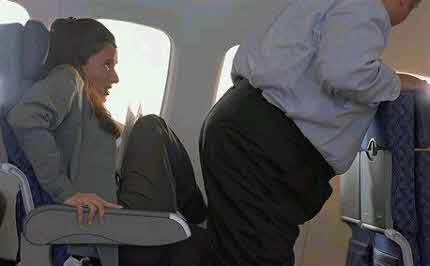
\includegraphics[width=7cm]{images/image009.png}
   \caption{With Airlines adding more and more seats to their planes, it is increasingly harder to maneuver around the cabin. 
                  Source: http://www.examiner.com/article/airlines-may-charge-fat-people-higher-fares}
  \label{fig:9}
\end{figure}


With the emergence of global business, people are constantly on the go today and airports are becoming larger and larger, growing more busy each year.  The distance from check-in to gate is increasing as more airlines expand routes and terminals grow.  As the airports grow, it becomes harder to make the travel distance between check-in and gate short and quick.  Therefore, it becomes a problem for passengers that have a hard time walking long distances or need assistance with bags or a wheelchair. More airport staff is needed to move the passengers with assistance needs, and often the staff is not trained in dealing with disabilities.  Airlines have such limited space in the cabin because of the increased amount of seats that the assistive devices have to be stored in the cargo hold, making them susceptible to damage.  The flying experience today is tailored to a person that has all of his/her mobility, leaving out those who do not have the mobility or have some impairment that requires additional time. However, 58 million Americans live with a disability, including 5.5 million military veterans. \cite{}

Would it not be great if the flying experience were individually tailored to a person’s needs? What is the cabin could be redesigned to improve the flying experience for the passengers with limited mobility as well as for the average passenger? Such design would create an experience that is comfortable; making the airline and aircraft manufacturer more popular among its customers because the final user, the passenger, is the one the plane is designed for.

\section{Problem Statement}
To make this problem more tangible and approachable, we broke the project into different focus areas:

\begin{list}{-}{}
  \item Current systems in use in the airport and on the airplane
  \item User's Needs
  \item User's Complaints
  \item Identification of Critical Users
\end{list}

The whole process (see Appendix A Diagram A1) was analyzed and current systems that are in use based on FAA and ADA regulations were researched to determine the gaps in the system.  The gaps helped identify possible user needs.  In addition, user interviews were conducted to determine more needs and used to focus exact needs that we could address with our solution.  The interviews enlightened us with complaints that the current users had and ideas on where possible innovation areas lay.

For our problem, two distinct groups of users were quickly identified, the flight crew and the passengers with limited mobility.   The passengers with limited mobility were a very straightforward user group as it was identified in the problem statement.  However, the flight crew is the user that will have to use the solution on an everyday or every flight basis.  Therefore, the ease of use and the inclusion into the flight crew tasks have to be considered in order to make the solution a success.

\section{Corporate Partner: Embraer}

\begin{figure}[h]
  \centering
     
\includegraphics[width=7cm]{images/image010.jpg}
  \label{fig:10}
\end{figure}

The corporate partner for this design project is Embraer.  Since 1969, Embraer has been involved in all aspects of the aviation field.  Embraer began with support from the Brazilian Government to produce military aircraft in addition to its small passenger planes.  Embraer then expanded to agricultural planes and later to commercial planes and business/private jets.  Embraer has over 5,000 aircraft operating in over 80 countries.  They are the market leader for commercial jets with fewer than 120 seats.  Embraer is interested in expanding its commercial market to larger commercial jets, in maintaining some of the best executive jets, and in entering new defense markets.

\section*{Corporate Liaison}
Luciana Ribeiro Monteiro \\
  Technology Development \\
  Embraer - SJK \\
  Phone: +55 12 3927 8576 \\
  luciana.monteiro@embraer.com.br

\section{The Design Team}
Team Embraer was assembled using the results of the Herrmann Brain Dominance Instrument (HBDI) to determine compatible thinking styles and personality traits. Additionally, Robert, Laura, and Cliff were all brought in at the beginning of winter quarter.  Our team has a diverse educational, cultural, and social background that encompasses many skill sets and multiple areas of study. 

\subsection*{Stanford University}

\begin{framed}
\noindent 
\includegraphics[width=40mm]{images/image011.jpg}
\parbox[b]{0.6\textwidth}{Marria Barrera\\
Status: Mechanical Engineering Graduate Student\\
Contact: mariab8@stanford.edu\\
}

I was born in Colombia and moved to South Florida with my mom when I was 10. My dad and sister still live in Colombia so I tend to hop back and forth every chance I get. I did my undergraduate at Stanford also in Mechanical Engineering and have developed a deep interest for entrepreneurship during my time here. I run a tutoring company in the area and hope to one day start a company in the aviation sector. I am also enjoy traveling, photography and playing with puppies.
\end{framed}

\begin{framed}
\noindent 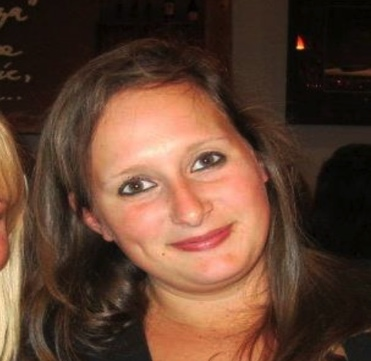
\includegraphics[width=40mm]{images/image012.jpg}
\parbox[b]{0.6\textwidth}{Erika Finley\\
Status: Mechanical Engineering Graduate Student\\
Contact: erikaf@stanford.edu\\
}

I was born and raised in Tennessee. I attended the University of Tennessee at Knoxville for my undergraduate degree in Mechanical Engineering.  I participated in a study abroad in Canberra, Australia.  I have interned for Tennessee Valley Authority at Browns Ferry Nuclear Plant and for Schlumberger at the Rosharon Design Center. I will be interning at Microsoft this upcoming summer. My interests include baking, reading, photography, and roller coasters.  
\end{framed}

\begin{framed}
\noindent 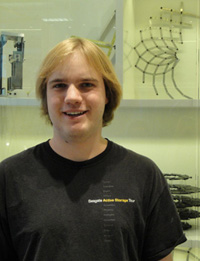
\includegraphics[width=40mm]{images/robert_karol.jpg}
\parbox[b]{0.6\textwidth}{Robert Karol\\
Status: Aeronautics and Astronautics Graduate Student\\
Contact: robkarol@stanford.edu \\
}

I grew up in New Jersey through high school. After that, I moved to southern california where I attended the California Institute of Technology majoring in Mechanical Engineering with minors in Aerospace Engineering and Control and Dynamical Systems. I have worked on robotics projects with NASA's Jet Propulsion Laboratory, as well as experiments in high altitude photography and performed research in microgravity.
\end{framed}

\begin{framed}
\noindent 
\includegraphics[width=40mm]{images/image012bis}
\parbox[b]{0.6\textwidth}{Laura Hoinville\\
Status: Aeronautics and Astronautics Graduate Student\\
Contact:  laurah31@stanford.edu \\
}

I come from Toulouse, France. I attended ISEA-Supaéro (the French Graduate school of Engineering) at Toulouse for my undergraduate degree in Aeronautics. I’ve worked at Airbus head quarters in Blagnac, France as an intern last summer and want to make a career in the field of aircraft design. I’m interested in dance (ballet, modern jazz, contemporary), gymnastics, scuba diving and reading.
\end{framed}

\begin{framed}
\noindent 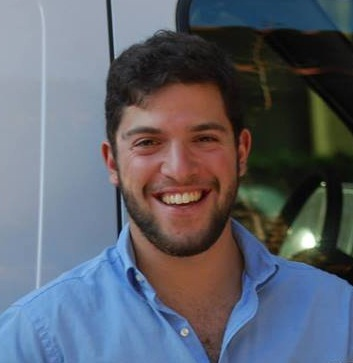
\includegraphics[width=40mm]{images/cliff.jpg}
\parbox[b]{0.6\textwidth}{Clifford Bargar\\
Status: Mechanical Engineering Graduate Student\\
Contact: cbargar@stanford.edu \\
Website: http://cliffbargar.com \\
}

Having spent the first 22 years of my life within a subway ride of Boston, Massachusetts, I decided to drive west and come to Stanford. I'm completing my MSME this spring, focusing on mechatronics, robotics, and controls. I graduated with a BSME from Tufts University, where I double majored in Mechanical Engineering and Mathematics, was an active member of the chapter of Engineers Without Borders and the Tufts Robotics Club, and ran on the Tufts Cross Country and Track and Field teams. I've spent the last several summers as a student research at the Wyss Institute for Bioinspired Engineering at Harvard University, MIT Lincoln Laboratory, and the Tufts Center for Engineering Education and Outreach.
\end{framed}

\subsection*{University of S\~{a}o Paulo}

\begin{framed}
\noindent 
\includegraphics[width=40mm]{images/image013}
\parbox[b]{0.6\textwidth}{Amanda Mota Almeida\\
Status: Product Design Graduate Student\\
Contact: amandamotaalmeida@gmail.com \\
}

I was born and raised in S\~{a}o Paulo. I'm attending the University of S\~{a}o Paulo for my undergraduate studies in Product and Graphic Design. I have worked in a project with Embraer in the past regarding the design and comfort in the aircraft cabin (2011), I have interned for Staples in S\~{a}o Paulo – SP (2012) and I was part of exchange in Portugal last year (2013). My interests include: photography, arts and crafts and reading.
\end{framed}

\begin{framed}
\noindent 
\includegraphics[width=40mm]{images/image014}
\parbox[b]{0.6\textwidth}{Rodrigo Monteiro de Aquino\\
Status: Computer Engineering Undergraduate Student \\
Contact:guigonyts@usp.br \\
}

I have lived all my life in S\~{a}o Paulo. I am now graduating in Computer Engineering at USP and I also work in a technology development lab at the university. I have worked on several projects developing educational games and other educational interfaces that help children learn with technological devices.  I like to play videogames and go to the movie theater. I like science fiction movies and reading adventure books.
\end{framed}

\begin{figure}[h]
  \centering
     
\includegraphics[width=7cm]{images/image014}
   \caption{With Airlines adding more and more seats to their planes, it is increasingly harder to maneuver around the cabin.
                  Source: http://www.examiner.com/article/airlines-may-charge-fat-people-higher-fares}
  \label{fig:14}
\end{figure}


\begin{figure}[h]
  \centering
     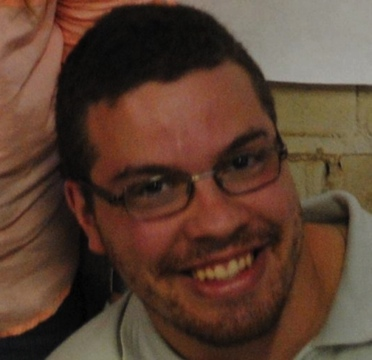
\includegraphics[width=7cm]{images/image015}
  \label{fig:15}
\end{figure}

\textbf{Luiz Durao}
Status: Industrial Engineering Undergraduate Student \\
Contact: luiz.durao@usp.br \\
I was born and raised in S\~{a}o Paulo city. I attended Colégio Etapa for my High School and it was while participating in the Chemistry and Physics Olympiads that I discovered my taste for the sciences. I'm attending the University of S\~{a}o Paulo for my undergraduate studies in Industrial Engineering. I have interned for GE Oil and Gas at Jandira – SP and I have worked since my sophomore year as a teaching assistant for some courses at USP. My interests include soccer, music and movies.

\begin{figure}[h]
  \centering
     
\includegraphics[width=7cm]{images/image016}
  \label{fig:16}
\end{figure}

\textbf{Guilherme Kok}
Status: Industrial Engineering Undergraduate Student \\
Contact: guilhermekok@gmail.com \\
Brazilian and a soccer enthusiast, I grew up in S\~{a}o Paulo and in Baltimore. I’ve also spent 5 months in Nanaimo (Canada, BC) and 1 year studying at the University of Illinois at Urbana Champaign. I’m currently finishing my undergraduate studies at the University of S\~{a}o Paulo in Brazil, where I study Industrial Engineering. I have interned for a taxi app startup and have done undergrad research concerning the consolidation of the phonographic industry. My interests include playing soccer, hiking, tasting different cuisines and travelling, preferably to remote locations. 

\section{Coaches}
a) Shelly Goldberg \\
Contact: shelly.goldberg@gmail.com \\ 
Shelly Goldberg was an ME310 alum from 2005, where her team worked on the EADS ?AugmenTable?.  Shelly has been at Apple, Inc. for the past 9 years since leaving Stanford.  She is now a Senior Manager in the Mac Product Design group, where she leads a team of mechanical and product design engineers responsible for conceiving, designing, engineering, producing, and sustaining the Mac portables and desktops.  

b) Annika Matta \\
Contact: annikamatta@gmail.com \\
Annika Matta is a former ME310 student and course assistant with a background in product and user experience design. As an ME310er she worked with SAP to build the Nib, a tablet with a writing experience reminiscent of paper. She graduated in 2013 and now works as a user interface designer at a consumer software startup in the Bay Area.
